\PassOptionsToPackage{xcolor}{usenames,dvipsnames,svgnames,table}
\documentclass[10pt]{report}
\usepackage[T1]{fontenc}
\usepackage{lmodern}
\usepackage{pdfcolmk}
\usepackage{multirow}
\usepackage{graphicx}
\usepackage{pifont}
\usepackage{amsmath,amsfonts,amsthm,amssymb}
\usepackage{setspace}
\usepackage{Tabbing}
\usepackage{etoolbox}
\usepackage{fancyhdr}
\usepackage{lastpage}
\usepackage{listings}
\usepackage{extramarks}
\usepackage{enumerate}
\usepackage{soul,color}
\usepackage{graphicx,float,wrapfig}
\usepackage{amsmath,amssymb,rotating}
\usepackage{epsfig}
\usepackage{color}
\usepackage{hyperref}
\usepackage{animate}
\usepackage{array}
\usepackage{graphics, color}
\usepackage{graphicx}
\usepackage{epsfig}
\usepackage{setspace}
\usepackage{verbatim}
\usepackage[margin=1.0in]{geometry}
\usepackage{tikz}
\usepackage{mdframed}
\usepackage{clrscode3e}
\usepackage{formalHW}
\usepackage[imouzon,none]{formatHW}
\usepackage{fancyquote}
\usepackage{fancyenvironments}
\usepackage{mymathmacros}
\usepackage{algorithm}
\usepackage[noend]{algpseudocode}
\usepackage{pgfplots}

%set up fancy page header
\pagestyle{fancy}
         \lhead{\href{mailto:imouzon@iastate.edu}{\nolinkurl{imouzon@iastate.edu}}}
            \lhead{imouzon}
      \chead{\href{mailto:DMC@ISU}{\nolinkurl{DMC@ISU}}\ (One Week Left,\ Spring 2015): Multiway LLR}  
   \rhead{\firstxmark}
   \lfoot{\lastxmark}
   \cfoot{}
   \rfoot{Page\ \thepage\ of\ \pageref{LastPage}}
   \renewcommand\headrulewidth{0.4pt}
   \renewcommand\footrulewidth{0.4pt}

% pandoc syntax highlighting
\usepackage{color}
\usepackage{fancyvrb}
\newcommand{\VerbBar}{|}
\newcommand{\VERB}{\Verb[commandchars=\\\{\}]}
\DefineVerbatimEnvironment{Highlighting}{Verbatim}{commandchars=\\\{\}}
% Add ',fontsize=\small' for more characters per line
\newenvironment{Shaded}{}{}
\newcommand{\KeywordTok}[1]{\textcolor[rgb]{0.00,0.44,0.13}{\textbf{{#1}}}}
\newcommand{\DataTypeTok}[1]{\textcolor[rgb]{0.56,0.13,0.00}{{#1}}}
\newcommand{\DecValTok}[1]{\textcolor[rgb]{0.25,0.63,0.44}{{#1}}}
\newcommand{\BaseNTok}[1]{\textcolor[rgb]{0.25,0.63,0.44}{{#1}}}
\newcommand{\FloatTok}[1]{\textcolor[rgb]{0.25,0.63,0.44}{{#1}}}
\newcommand{\CharTok}[1]{\textcolor[rgb]{0.25,0.44,0.63}{{#1}}}
\newcommand{\StringTok}[1]{\textcolor[rgb]{0.25,0.44,0.63}{{#1}}}
\newcommand{\CommentTok}[1]{\textcolor[rgb]{0.38,0.63,0.69}{\textit{{#1}}}}
\newcommand{\OtherTok}[1]{\textcolor[rgb]{0.00,0.44,0.13}{{#1}}}
\newcommand{\AlertTok}[1]{\textcolor[rgb]{1.00,0.00,0.00}{\textbf{{#1}}}}
\newcommand{\FunctionTok}[1]{\textcolor[rgb]{0.02,0.16,0.49}{{#1}}}
\newcommand{\RegionMarkerTok}[1]{{#1}}
\newcommand{\ErrorTok}[1]{\textcolor[rgb]{1.00,0.00,0.00}{\textbf{{#1}}}}
\newcommand{\NormalTok}[1]{{#1}}

% header includes

\begin{document}

\thispagestyle{empty}%
\begin{center}%
    \renewcommand{\arraystretch}{1.5}%
    \begin{tabular}{c}%
       \Large{\href{mailto:DMC@ISU}{\nolinkurl{DMC@ISU}}: Iowa State University's 2015 Data Mining Cup Team}\\
       Multiway Comparisons\\
       Spring 2015, One Week Left \\
    \end{tabular}
\end{center}

\begin{center}
 \renewcommand{\arraystretch}{1.5}
 \begin{tabular*}{0.65\textwidth}{r@{:\hspace{.3cm}}l}
    \hline
     Name& Pete and Ian\\
     email& \href{mailto:imouzon@iastate.edu}{\nolinkurl{imouzon@iastate.edu}}\\
    
    
     Due Date&  May 13, 2015\\
    \hline
 \end{tabular*}
\end{center}

I am using the following packages:

\begin{Shaded}
\begin{Highlighting}[]
   \KeywordTok{library}\NormalTok{(magrittr)}
   \KeywordTok{library}\NormalTok{(dplyr)}
   \KeywordTok{library}\NormalTok{(tidyr)}
   \KeywordTok{library}\NormalTok{(lubridate)}
   \KeywordTok{library}\NormalTok{(ggplot2)}
   \KeywordTok{library}\NormalTok{(rCharts)}
   \KeywordTok{library}\NormalTok{(xtable)}
   \KeywordTok{library}\NormalTok{(foreach)}
   \KeywordTok{library}\NormalTok{(gtools)}
   \KeywordTok{library}\NormalTok{(knitr)}
   \KeywordTok{library}\NormalTok{(utils)}
   \KeywordTok{source}\NormalTok{(}\StringTok{"~/dmc2015/ian/R/renm.R"}\NormalTok{)}
\end{Highlighting}
\end{Shaded}

\section{Loglikelihood statistics}\label{loglikelihood-statistics}

\begin{Shaded}
\begin{Highlighting}[]
\KeywordTok{source}\NormalTok{(}\StringTok{"./R/llr_multiway.R"}\NormalTok{)}
\end{Highlighting}
\end{Shaded}

\section{Getting Tranthe Data and
Manipulations}\label{getting-tranthe-data-and-manipulations}

I am using our new clean data - so should you

I can melt the columns by coupon using the following:

\begin{verbatim}
## using the following as id:
##  orderID,
##  orderTime,
##  userID,
##  couponsReceived,
##  basketValue,
##  couponsReceivedDate,
##  couponsReceivedTime,
##  couponsReceivedDoW,
##  couponsReceivedWeekend,
##  couponsReceivedFriSat,
##  orderTimeDate,
##  orderTimeTime,
##  orderTimeDoW,
##  orderTimeWeekend,
##  orderTimeFriSat,
##  batchID,
##  couponsExpire,
##  couponsSent,
##  TimeBtwnSentRec,
##  TimeBtwnRecExpire,
##  TimeBtwnRecOrder,
##  TimeBtwnOrderExpire
## 
## using the following as measure columns:
##  couponID1,
##  price1,
##  basePrice1,
##  reward1,
##  premiumProduct1,
##  brand1,
##  productGroup1,
##  categoryIDs1,
##  coupon1Used,
##  couponID2,
##  price2,
##  basePrice2,
##  reward2,
##  premiumProduct2,
##  brand2,
##  productGroup2,
##  categoryIDs2,
##  coupon2Used,
##  couponID3,
##  price3,
##  basePrice3,
##  reward3,
##  premiumProduct3,
##  brand3,
##  productGroup3,
##  categoryIDs3,
##  coupon3Used
\end{verbatim}

\subsection{Make a few quick features}\label{make-a-few-quick-features}

I and can split the columns of product group using:

\begin{verbatim}
## Loading required package: tcltk
\end{verbatim}

\section{Based on Historical Set 1}\label{based-on-historical-set-1}

\begin{Shaded}
\begin{Highlighting}[]
\NormalTok{HTVset3 =}\StringTok{ }\KeywordTok{readRDS}\NormalTok{(}\StringTok{"~/dmc2015/data/featureMatrix/HTVset3.rds"}\NormalTok{)}
\KeywordTok{names}\NormalTok{(dm)}
\end{Highlighting}
\end{Shaded}

\begin{verbatim}
##  [1] "orderID"                "orderTime"             
##  [3] "userID"                 "couponsReceived"       
##  [5] "basketValue"            "couponsReceivedDate"   
##  [7] "couponsReceivedTime"    "couponsReceivedDoW"    
##  [9] "couponsReceivedWeekend" "couponsReceivedFriSat" 
## [11] "orderTimeDate"          "orderTimeTime"         
## [13] "orderTimeDoW"           "orderTimeWeekend"      
## [15] "orderTimeFriSat"        "batchID"               
## [17] "couponsExpire"          "couponsSent"           
## [19] "TimeBtwnSentRec"        "TimeBtwnRecExpire"     
## [21] "TimeBtwnRecOrder"       "TimeBtwnOrderExpire"   
## [23] "couponID"               "price"                 
## [25] "basePrice"              "reward"                
## [27] "premiumProduct"         "brand"                 
## [29] "productGroup"           "categoryIDs"           
## [31] "couponUsed"             "couponCol"             
## [33] "ShopFast"               "EarlyRec"              
## [35] "Shop60"                 "Shop30"                
## [37] "Shop15"                 "RecExpire60"           
## [39] "RecOrder60"             "OrderExpire60"         
## [41] "basePrice_price_ratio"
\end{verbatim}

\subsection{Making comparisons}\label{making-comparisons}

Using these likelihoods, we can make the following comparisons:
\textbf{basePrice\_price\_ratio, reward}

\begin{Shaded}
\begin{Highlighting}[]
\NormalTok{colsel =}\StringTok{ }\KeywordTok{which}\NormalTok{(}\KeywordTok{names}\NormalTok{(dm) %in%}\StringTok{ }\KeywordTok{c}\NormalTok{(}\StringTok{"basePrice_price_ratio"}\NormalTok{, }\StringTok{"reward"}\NormalTok{))}
\NormalTok{result =}\StringTok{ }\KeywordTok{llr_multiway}\NormalTok{(dm, HTVset3$H, colsel)}

\NormalTok{dm %>%}\StringTok{ }\KeywordTok{left_join}\NormalTok{(result$long, }\DataTypeTok{by =} \KeywordTok{c}\NormalTok{(}\StringTok{"orderID"}\NormalTok{, }\StringTok{"couponCol"}\NormalTok{)) %>%}\StringTok{ }\KeywordTok{ggplot}\NormalTok{(}\KeywordTok{aes}\NormalTok{(}\KeywordTok{factor}\NormalTok{(reward), }
    \NormalTok{llr_naive_rwdXbasePrice_price_ratio, }\DataTypeTok{color =} \KeywordTok{factor}\NormalTok{(couponUsed), }\DataTypeTok{group =} \NormalTok{couponCol)) +}\StringTok{ }
\StringTok{    }\KeywordTok{geom_boxplot}\NormalTok{()}

\CommentTok{# show long results}
\KeywordTok{tail}\NormalTok{(result$long) %>%}\StringTok{ }\NormalTok{kable}
\end{Highlighting}
\end{Shaded}

\begin{longtable}[c]{@{}lrrrrrrr@{}}
\toprule
& orderID & couponCol & ntimes\_rwdXbasePrice\_price\_ratio &
timesUsed\_rwdXbasePrice\_price\_ratio &
timesNotUsed\_rwdXbasePrice\_price\_ratio &
llr\_est\_rwdXbasePrice\_price\_ratio &
llr\_naive\_rwdXbasePrice\_price\_ratio\tabularnewline
\midrule
\endhead
20161 & 6721 & 1 & 27 & 10 & 17 & -0.5898659 & -0.4924765\tabularnewline
20162 & 6721 & 2 & 36 & 3 & 33 & -2.3121781 & -2.1400662\tabularnewline
20163 & 6721 & 3 & 7 & 0 & 7 & -2.9747989 & -2.0794415\tabularnewline
20164 & 6722 & 1 & 47 & 7 & 40 & -1.7256751 & -1.6341305\tabularnewline
20165 & 6722 & 2 & 6 & 0 & 6 & -2.8549347 & -1.9459101\tabularnewline
20166 & 6722 & 3 & 14 & 3 & 11 & -1.3146044 & -1.0986123\tabularnewline
\bottomrule
\end{longtable}

\begin{Shaded}
\begin{Highlighting}[]
\CommentTok{# show wide results}
\KeywordTok{head}\NormalTok{(result$wide) %>%}\StringTok{ }\NormalTok{kable}
\end{Highlighting}
\end{Shaded}

\begin{longtable}[c]{@{}rrrrrrrrrrrrrrrr@{}}
\toprule
orderID & ntimes\_rwdXbasePrice\_price\_ratio\_col1 &
ntimes\_rwdXbasePrice\_price\_ratio\_col2 &
ntimes\_rwdXbasePrice\_price\_ratio\_col3 &
timesUsed\_rwdXbasePrice\_price\_ratio\_col1 &
timesUsed\_rwdXbasePrice\_price\_ratio\_col2 &
timesUsed\_rwdXbasePrice\_price\_ratio\_col3 &
timesNotUsed\_rwdXbasePrice\_price\_ratio\_col1 &
timesNotUsed\_rwdXbasePrice\_price\_ratio\_col2 &
timesNotUsed\_rwdXbasePrice\_price\_ratio\_col3 &
llr\_est\_rwdXbasePrice\_price\_ratio\_col1 &
llr\_est\_rwdXbasePrice\_price\_ratio\_col2 &
llr\_est\_rwdXbasePrice\_price\_ratio\_col3 &
llr\_naive\_rwdXbasePrice\_price\_ratio\_col1 &
llr\_naive\_rwdXbasePrice\_price\_ratio\_col2 &
llr\_naive\_rwdXbasePrice\_price\_ratio\_col3\tabularnewline
\midrule
\endhead
1 & 14 & 4 & 67 & 3 & 2 & 7 & 11 & 2 & 60 & -1.3146044 & -0.4518853 &
-2.1162741 & -1.0986123 & 0.000000 & -2.0314323\tabularnewline
2 & 1 & 38 & 1 & 1 & 9 & 1 & 0 & 29 & 0 & -0.2437339 & -1.1829997 &
-0.2437339 & 0.6931472 & -1.098612 & 0.6931472\tabularnewline
3 & 104 & 104 & 14 & 24 & 24 & 3 & 80 & 80 & 11 & -1.2082100 &
-1.2082100 & -1.3146044 & -1.1755733 & -1.175573 &
-1.0986123\tabularnewline
4 & 13 & 56 & 5 & 4 & 6 & 1 & 9 & 50 & 4 & -0.8910657 & -2.0840178 &
-1.3939705 & -0.6931472 & -1.985915 & -0.9162907\tabularnewline
5 & 27 & 21 & 8 & 4 & 0 & 2 & 23 & 21 & 6 & -1.7196151 & -3.9231415 &
-1.1639605 & -1.5686159 & -3.091042 & -0.8472979\tabularnewline
6 & 26 & 10 & 3 & 9 & 0 & 1 & 17 & 10 & 2 & -0.6904328 & -3.2666303 &
-0.9758470 & -0.5877867 & -2.397895 & -0.4054651\tabularnewline
\bottomrule
\end{longtable}

\begin{center}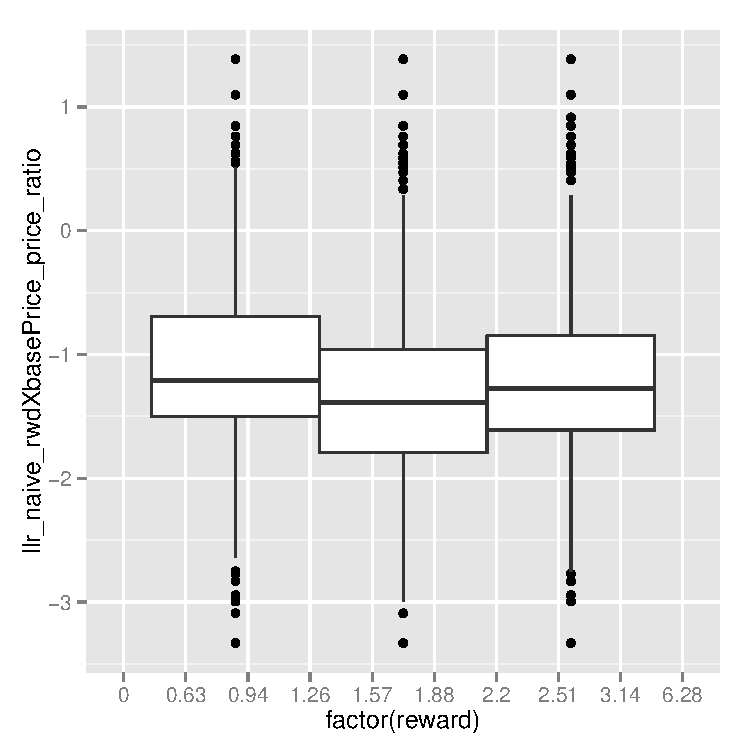
\includegraphics{/Users/user/dmc2015/ian/graphics/fig_unnamed-chunk-4-1} \end{center}

Make this a function:

\begin{Shaded}
\begin{Highlighting}[]
\NormalTok{CreateSets =}\StringTok{ }\NormalTok{function(varns) \{}
    \NormalTok{filename =}\StringTok{ }\KeywordTok{paste}\NormalTok{(varns, }\DataTypeTok{collapse =} \StringTok{"X"}\NormalTok{)}
    \NormalTok{colsel =}\StringTok{ }\KeywordTok{which}\NormalTok{(}\KeywordTok{names}\NormalTok{(dm) %in%}\StringTok{ }\NormalTok{varns)}
    
    \KeywordTok{message}\NormalTok{(}\StringTok{"Now making llrs for "}\NormalTok{, filename)}
    \NormalTok{result =}\StringTok{ }\KeywordTok{llr_multiway}\NormalTok{(dm, HTVset3$H, colsel)}
    
    \CommentTok{# save long results}
    \NormalTok{result$long %>%}\StringTok{ }\KeywordTok{saveRDS}\NormalTok{(}\DataTypeTok{file =} \KeywordTok{paste0}\NormalTok{(}\StringTok{"~/dmc2015/features/feature_files/set3/llr_"}\NormalTok{, }
        \NormalTok{filename, }\StringTok{"_long.rds"}\NormalTok{))}
    
    \CommentTok{# save wide results}
    \NormalTok{result$wide %>%}\StringTok{ }\KeywordTok{saveRDS}\NormalTok{(}\DataTypeTok{file =} \KeywordTok{paste0}\NormalTok{(}\StringTok{"~/dmc2015/features/feature_files/set3/llr_"}\NormalTok{, }
        \NormalTok{filename, }\StringTok{"_wide.rds"}\NormalTok{))}
\NormalTok{\}}
\end{Highlighting}
\end{Shaded}

\subsection{Choosing comparisons}\label{choosing-comparisons}

\begin{Shaded}
\begin{Highlighting}[]
\CommentTok{# comparison groups}
\NormalTok{groupA =}\StringTok{ }\KeywordTok{c}\NormalTok{(}\StringTok{"Shop60"}\NormalTok{, }\StringTok{"Shop30"}\NormalTok{, }\StringTok{"Shop15"}\NormalTok{, }\StringTok{"RecExpire60"}\NormalTok{, }\StringTok{"RecOrder60"}\NormalTok{, }\StringTok{"OrderExpire60"}\NormalTok{)}

\NormalTok{groupB =}\StringTok{ }\KeywordTok{c}\NormalTok{(}\StringTok{"basePrice_price_ratio"}\NormalTok{, }\StringTok{"price"}\NormalTok{, }\StringTok{"basePrice"}\NormalTok{)}

\NormalTok{groupC2 =}\StringTok{ "couponID"}

\NormalTok{groupD1 =}\StringTok{ }\KeywordTok{c}\NormalTok{(}\StringTok{"ShopFast"}\NormalTok{, }\StringTok{"EarlyRec"}\NormalTok{)}
\NormalTok{groupD2 =}\StringTok{ }\KeywordTok{c}\NormalTok{(}\StringTok{"premiumProduct"}\NormalTok{, }\StringTok{"brand"}\NormalTok{, }\StringTok{"productGroup"}\NormalTok{, }\StringTok{"categoryIDs"}\NormalTok{, }\StringTok{"reward"}\NormalTok{)}
\end{Highlighting}
\end{Shaded}

\section{One way Comparisons}\label{one-way-comparisons}

\begin{Shaded}
\begin{Highlighting}[]
\CommentTok{# one way}
\NormalTok{oneway =}\StringTok{ }\KeywordTok{c}\NormalTok{(groupA, groupB, groupC2, groupD1, groupD2)}
\KeywordTok{sapply}\NormalTok{(oneway, function(i) }\KeywordTok{CreateSets}\NormalTok{(i))}
\end{Highlighting}
\end{Shaded}

\begin{verbatim}
## Now making llrs for Shop60
## Now making llrs for Shop30
## Now making llrs for Shop15
## Now making llrs for RecExpire60
## Now making llrs for RecOrder60
## Now making llrs for OrderExpire60
## Now making llrs for basePrice_price_ratio
## Now making llrs for price
## Now making llrs for basePrice
## Now making llrs for couponID
## Now making llrs for ShopFast
## Now making llrs for EarlyRec
## Now making llrs for premiumProduct
## Now making llrs for brand
## Now making llrs for productGroup
## Now making llrs for categoryIDs
## Now making llrs for reward
\end{verbatim}

\begin{verbatim}
## $Shop60
## NULL
## 
## $Shop30
## NULL
## 
## $Shop15
## NULL
## 
## $RecExpire60
## NULL
## 
## $RecOrder60
## NULL
## 
## $OrderExpire60
## NULL
## 
## $basePrice_price_ratio
## NULL
## 
## $price
## NULL
## 
## $basePrice
## NULL
## 
## $couponID
## NULL
## 
## $ShopFast
## NULL
## 
## $EarlyRec
## NULL
## 
## $premiumProduct
## NULL
## 
## $brand
## NULL
## 
## $productGroup
## NULL
## 
## $categoryIDs
## NULL
## 
## $reward
## NULL
\end{verbatim}

\section{Two Way Comparisons}\label{two-way-comparisons}

\begin{Shaded}
\begin{Highlighting}[]
\NormalTok{## two way}
\NormalTok{twoway =}\StringTok{ }\KeywordTok{combn}\NormalTok{(}\KeywordTok{c}\NormalTok{(groupB, groupD1, groupD2), }\DecValTok{2}\NormalTok{) %>%}\StringTok{ }\KeywordTok{cbind}\NormalTok{(}\KeywordTok{combn}\NormalTok{(}\KeywordTok{c}\NormalTok{(groupC2, groupD1), }
    \DecValTok{2}\NormalTok{))}
\KeywordTok{sapply}\NormalTok{(}\DecValTok{1}\NormalTok{:}\KeywordTok{ncol}\NormalTok{(twoway), function(i) }\KeywordTok{CreateSets}\NormalTok{(twoway[, i]))}
\end{Highlighting}
\end{Shaded}

\begin{verbatim}
## Now making llrs for basePrice_price_ratioXprice
## Now making llrs for basePrice_price_ratioXbasePrice
## Now making llrs for basePrice_price_ratioXShopFast
## Now making llrs for basePrice_price_ratioXEarlyRec
## Now making llrs for basePrice_price_ratioXpremiumProduct
## Now making llrs for basePrice_price_ratioXbrand
## Now making llrs for basePrice_price_ratioXproductGroup
## Now making llrs for basePrice_price_ratioXcategoryIDs
## Now making llrs for basePrice_price_ratioXreward
## Now making llrs for priceXbasePrice
## Now making llrs for priceXShopFast
## Now making llrs for priceXEarlyRec
## Now making llrs for priceXpremiumProduct
## Now making llrs for priceXbrand
## Now making llrs for priceXproductGroup
## Now making llrs for priceXcategoryIDs
## Now making llrs for priceXreward
## Now making llrs for basePriceXShopFast
## Now making llrs for basePriceXEarlyRec
## Now making llrs for basePriceXpremiumProduct
## Now making llrs for basePriceXbrand
## Now making llrs for basePriceXproductGroup
## Now making llrs for basePriceXcategoryIDs
## Now making llrs for basePriceXreward
## Now making llrs for ShopFastXEarlyRec
## Now making llrs for ShopFastXpremiumProduct
## Now making llrs for ShopFastXbrand
## Now making llrs for ShopFastXproductGroup
## Now making llrs for ShopFastXcategoryIDs
## Now making llrs for ShopFastXreward
## Now making llrs for EarlyRecXpremiumProduct
## Now making llrs for EarlyRecXbrand
## Now making llrs for EarlyRecXproductGroup
## Now making llrs for EarlyRecXcategoryIDs
## Now making llrs for EarlyRecXreward
## Now making llrs for premiumProductXbrand
## Now making llrs for premiumProductXproductGroup
## Now making llrs for premiumProductXcategoryIDs
## Now making llrs for premiumProductXreward
## Now making llrs for brandXproductGroup
## Now making llrs for brandXcategoryIDs
## Now making llrs for brandXreward
## Now making llrs for productGroupXcategoryIDs
## Now making llrs for productGroupXreward
## Now making llrs for categoryIDsXreward
## Now making llrs for couponIDXShopFast
## Now making llrs for couponIDXEarlyRec
## Now making llrs for ShopFastXEarlyRec
\end{verbatim}

\begin{verbatim}
## [[1]]
## NULL
## 
## [[2]]
## NULL
## 
## [[3]]
## NULL
## 
## [[4]]
## NULL
## 
## [[5]]
## NULL
## 
## [[6]]
## NULL
## 
## [[7]]
## NULL
## 
## [[8]]
## NULL
## 
## [[9]]
## NULL
## 
## [[10]]
## NULL
## 
## [[11]]
## NULL
## 
## [[12]]
## NULL
## 
## [[13]]
## NULL
## 
## [[14]]
## NULL
## 
## [[15]]
## NULL
## 
## [[16]]
## NULL
## 
## [[17]]
## NULL
## 
## [[18]]
## NULL
## 
## [[19]]
## NULL
## 
## [[20]]
## NULL
## 
## [[21]]
## NULL
## 
## [[22]]
## NULL
## 
## [[23]]
## NULL
## 
## [[24]]
## NULL
## 
## [[25]]
## NULL
## 
## [[26]]
## NULL
## 
## [[27]]
## NULL
## 
## [[28]]
## NULL
## 
## [[29]]
## NULL
## 
## [[30]]
## NULL
## 
## [[31]]
## NULL
## 
## [[32]]
## NULL
## 
## [[33]]
## NULL
## 
## [[34]]
## NULL
## 
## [[35]]
## NULL
## 
## [[36]]
## NULL
## 
## [[37]]
## NULL
## 
## [[38]]
## NULL
## 
## [[39]]
## NULL
## 
## [[40]]
## NULL
## 
## [[41]]
## NULL
## 
## [[42]]
## NULL
## 
## [[43]]
## NULL
## 
## [[44]]
## NULL
## 
## [[45]]
## NULL
## 
## [[46]]
## NULL
## 
## [[47]]
## NULL
## 
## [[48]]
## NULL
\end{verbatim}

\section{Three Way Comparisons}\label{three-way-comparisons}

\begin{Shaded}
\begin{Highlighting}[]
\NormalTok{## three way}
\NormalTok{threeway =}\StringTok{ }\KeywordTok{combn}\NormalTok{(}\KeywordTok{c}\NormalTok{(groupB), }\DecValTok{3}\NormalTok{) %>%}\StringTok{ }\KeywordTok{cbind}\NormalTok{(}\KeywordTok{do.call}\NormalTok{(}\StringTok{"cbind"}\NormalTok{, }\KeywordTok{lapply}\NormalTok{(groupB, function(x) }\KeywordTok{combn}\NormalTok{(}\KeywordTok{c}\NormalTok{(x, }
    \NormalTok{groupD1, groupD2), }\DecValTok{3}\NormalTok{)))) %>%}\StringTok{ }\KeywordTok{cbind}\NormalTok{(}\KeywordTok{do.call}\NormalTok{(}\StringTok{"cbind"}\NormalTok{, }\KeywordTok{lapply}\NormalTok{(}\KeywordTok{c}\NormalTok{(groupD1, groupD2), }
    \NormalTok{function(x) }\KeywordTok{combn}\NormalTok{(}\KeywordTok{c}\NormalTok{(x, groupB), }\DecValTok{3}\NormalTok{)))) %>%}\StringTok{ }\KeywordTok{cbind}\NormalTok{(}\KeywordTok{combn}\NormalTok{(}\KeywordTok{c}\NormalTok{(groupD1, groupD2), }
    \DecValTok{3}\NormalTok{))}
\KeywordTok{sapply}\NormalTok{(}\DecValTok{1}\NormalTok{:}\KeywordTok{ncol}\NormalTok{(threeway), function(i) }\KeywordTok{CreateSets}\NormalTok{(threeway[, i]))}
\end{Highlighting}
\end{Shaded}

\begin{verbatim}
## Now making llrs for basePrice_price_ratioXpriceXbasePrice
## Now making llrs for basePrice_price_ratioXShopFastXEarlyRec
## Now making llrs for basePrice_price_ratioXShopFastXpremiumProduct
## Now making llrs for basePrice_price_ratioXShopFastXbrand
## Now making llrs for basePrice_price_ratioXShopFastXproductGroup
## Now making llrs for basePrice_price_ratioXShopFastXcategoryIDs
## Now making llrs for basePrice_price_ratioXShopFastXreward
## Now making llrs for basePrice_price_ratioXEarlyRecXpremiumProduct
## Now making llrs for basePrice_price_ratioXEarlyRecXbrand
## Now making llrs for basePrice_price_ratioXEarlyRecXproductGroup
## Now making llrs for basePrice_price_ratioXEarlyRecXcategoryIDs
## Now making llrs for basePrice_price_ratioXEarlyRecXreward
## Now making llrs for basePrice_price_ratioXpremiumProductXbrand
## Now making llrs for basePrice_price_ratioXpremiumProductXproductGroup
## Now making llrs for basePrice_price_ratioXpremiumProductXcategoryIDs
## Now making llrs for basePrice_price_ratioXpremiumProductXreward
## Now making llrs for basePrice_price_ratioXbrandXproductGroup
## Now making llrs for basePrice_price_ratioXbrandXcategoryIDs
## Now making llrs for basePrice_price_ratioXbrandXreward
## Now making llrs for basePrice_price_ratioXproductGroupXcategoryIDs
## Now making llrs for basePrice_price_ratioXproductGroupXreward
## Now making llrs for basePrice_price_ratioXcategoryIDsXreward
## Now making llrs for ShopFastXEarlyRecXpremiumProduct
## Now making llrs for ShopFastXEarlyRecXbrand
## Now making llrs for ShopFastXEarlyRecXproductGroup
## Now making llrs for ShopFastXEarlyRecXcategoryIDs
## Now making llrs for ShopFastXEarlyRecXreward
## Now making llrs for ShopFastXpremiumProductXbrand
## Now making llrs for ShopFastXpremiumProductXproductGroup
## Now making llrs for ShopFastXpremiumProductXcategoryIDs
## Now making llrs for ShopFastXpremiumProductXreward
## Now making llrs for ShopFastXbrandXproductGroup
## Now making llrs for ShopFastXbrandXcategoryIDs
## Now making llrs for ShopFastXbrandXreward
## Now making llrs for ShopFastXproductGroupXcategoryIDs
## Now making llrs for ShopFastXproductGroupXreward
## Now making llrs for ShopFastXcategoryIDsXreward
## Now making llrs for EarlyRecXpremiumProductXbrand
## Now making llrs for EarlyRecXpremiumProductXproductGroup
## Now making llrs for EarlyRecXpremiumProductXcategoryIDs
## Now making llrs for EarlyRecXpremiumProductXreward
## Now making llrs for EarlyRecXbrandXproductGroup
## Now making llrs for EarlyRecXbrandXcategoryIDs
## Now making llrs for EarlyRecXbrandXreward
## Now making llrs for EarlyRecXproductGroupXcategoryIDs
## Now making llrs for EarlyRecXproductGroupXreward
## Now making llrs for EarlyRecXcategoryIDsXreward
## Now making llrs for premiumProductXbrandXproductGroup
## Now making llrs for premiumProductXbrandXcategoryIDs
## Now making llrs for premiumProductXbrandXreward
## Now making llrs for premiumProductXproductGroupXcategoryIDs
## Now making llrs for premiumProductXproductGroupXreward
## Now making llrs for premiumProductXcategoryIDsXreward
## Now making llrs for brandXproductGroupXcategoryIDs
## Now making llrs for brandXproductGroupXreward
## Now making llrs for brandXcategoryIDsXreward
## Now making llrs for productGroupXcategoryIDsXreward
## Now making llrs for priceXShopFastXEarlyRec
## Now making llrs for priceXShopFastXpremiumProduct
## Now making llrs for priceXShopFastXbrand
## Now making llrs for priceXShopFastXproductGroup
## Now making llrs for priceXShopFastXcategoryIDs
## Now making llrs for priceXShopFastXreward
## Now making llrs for priceXEarlyRecXpremiumProduct
## Now making llrs for priceXEarlyRecXbrand
## Now making llrs for priceXEarlyRecXproductGroup
## Now making llrs for priceXEarlyRecXcategoryIDs
## Now making llrs for priceXEarlyRecXreward
## Now making llrs for priceXpremiumProductXbrand
## Now making llrs for priceXpremiumProductXproductGroup
## Now making llrs for priceXpremiumProductXcategoryIDs
## Now making llrs for priceXpremiumProductXreward
## Now making llrs for priceXbrandXproductGroup
## Now making llrs for priceXbrandXcategoryIDs
## Now making llrs for priceXbrandXreward
## Now making llrs for priceXproductGroupXcategoryIDs
## Now making llrs for priceXproductGroupXreward
## Now making llrs for priceXcategoryIDsXreward
## Now making llrs for ShopFastXEarlyRecXpremiumProduct
## Now making llrs for ShopFastXEarlyRecXbrand
## Now making llrs for ShopFastXEarlyRecXproductGroup
## Now making llrs for ShopFastXEarlyRecXcategoryIDs
## Now making llrs for ShopFastXEarlyRecXreward
## Now making llrs for ShopFastXpremiumProductXbrand
## Now making llrs for ShopFastXpremiumProductXproductGroup
## Now making llrs for ShopFastXpremiumProductXcategoryIDs
## Now making llrs for ShopFastXpremiumProductXreward
## Now making llrs for ShopFastXbrandXproductGroup
## Now making llrs for ShopFastXbrandXcategoryIDs
## Now making llrs for ShopFastXbrandXreward
## Now making llrs for ShopFastXproductGroupXcategoryIDs
## Now making llrs for ShopFastXproductGroupXreward
## Now making llrs for ShopFastXcategoryIDsXreward
## Now making llrs for EarlyRecXpremiumProductXbrand
## Now making llrs for EarlyRecXpremiumProductXproductGroup
## Now making llrs for EarlyRecXpremiumProductXcategoryIDs
## Now making llrs for EarlyRecXpremiumProductXreward
## Now making llrs for EarlyRecXbrandXproductGroup
## Now making llrs for EarlyRecXbrandXcategoryIDs
## Now making llrs for EarlyRecXbrandXreward
## Now making llrs for EarlyRecXproductGroupXcategoryIDs
## Now making llrs for EarlyRecXproductGroupXreward
## Now making llrs for EarlyRecXcategoryIDsXreward
## Now making llrs for premiumProductXbrandXproductGroup
## Now making llrs for premiumProductXbrandXcategoryIDs
## Now making llrs for premiumProductXbrandXreward
## Now making llrs for premiumProductXproductGroupXcategoryIDs
## Now making llrs for premiumProductXproductGroupXreward
## Now making llrs for premiumProductXcategoryIDsXreward
## Now making llrs for brandXproductGroupXcategoryIDs
## Now making llrs for brandXproductGroupXreward
## Now making llrs for brandXcategoryIDsXreward
## Now making llrs for productGroupXcategoryIDsXreward
## Now making llrs for basePriceXShopFastXEarlyRec
## Now making llrs for basePriceXShopFastXpremiumProduct
## Now making llrs for basePriceXShopFastXbrand
## Now making llrs for basePriceXShopFastXproductGroup
## Now making llrs for basePriceXShopFastXcategoryIDs
## Now making llrs for basePriceXShopFastXreward
## Now making llrs for basePriceXEarlyRecXpremiumProduct
## Now making llrs for basePriceXEarlyRecXbrand
## Now making llrs for basePriceXEarlyRecXproductGroup
## Now making llrs for basePriceXEarlyRecXcategoryIDs
## Now making llrs for basePriceXEarlyRecXreward
## Now making llrs for basePriceXpremiumProductXbrand
## Now making llrs for basePriceXpremiumProductXproductGroup
## Now making llrs for basePriceXpremiumProductXcategoryIDs
## Now making llrs for basePriceXpremiumProductXreward
## Now making llrs for basePriceXbrandXproductGroup
## Now making llrs for basePriceXbrandXcategoryIDs
## Now making llrs for basePriceXbrandXreward
## Now making llrs for basePriceXproductGroupXcategoryIDs
## Now making llrs for basePriceXproductGroupXreward
## Now making llrs for basePriceXcategoryIDsXreward
## Now making llrs for ShopFastXEarlyRecXpremiumProduct
## Now making llrs for ShopFastXEarlyRecXbrand
## Now making llrs for ShopFastXEarlyRecXproductGroup
## Now making llrs for ShopFastXEarlyRecXcategoryIDs
## Now making llrs for ShopFastXEarlyRecXreward
## Now making llrs for ShopFastXpremiumProductXbrand
## Now making llrs for ShopFastXpremiumProductXproductGroup
## Now making llrs for ShopFastXpremiumProductXcategoryIDs
## Now making llrs for ShopFastXpremiumProductXreward
## Now making llrs for ShopFastXbrandXproductGroup
## Now making llrs for ShopFastXbrandXcategoryIDs
## Now making llrs for ShopFastXbrandXreward
## Now making llrs for ShopFastXproductGroupXcategoryIDs
## Now making llrs for ShopFastXproductGroupXreward
## Now making llrs for ShopFastXcategoryIDsXreward
## Now making llrs for EarlyRecXpremiumProductXbrand
## Now making llrs for EarlyRecXpremiumProductXproductGroup
## Now making llrs for EarlyRecXpremiumProductXcategoryIDs
## Now making llrs for EarlyRecXpremiumProductXreward
## Now making llrs for EarlyRecXbrandXproductGroup
## Now making llrs for EarlyRecXbrandXcategoryIDs
## Now making llrs for EarlyRecXbrandXreward
## Now making llrs for EarlyRecXproductGroupXcategoryIDs
## Now making llrs for EarlyRecXproductGroupXreward
## Now making llrs for EarlyRecXcategoryIDsXreward
## Now making llrs for premiumProductXbrandXproductGroup
## Now making llrs for premiumProductXbrandXcategoryIDs
## Now making llrs for premiumProductXbrandXreward
## Now making llrs for premiumProductXproductGroupXcategoryIDs
## Now making llrs for premiumProductXproductGroupXreward
## Now making llrs for premiumProductXcategoryIDsXreward
## Now making llrs for brandXproductGroupXcategoryIDs
## Now making llrs for brandXproductGroupXreward
## Now making llrs for brandXcategoryIDsXreward
## Now making llrs for productGroupXcategoryIDsXreward
## Now making llrs for ShopFastXbasePrice_price_ratioXprice
## Now making llrs for ShopFastXbasePrice_price_ratioXbasePrice
## Now making llrs for ShopFastXpriceXbasePrice
## Now making llrs for basePrice_price_ratioXpriceXbasePrice
## Now making llrs for EarlyRecXbasePrice_price_ratioXprice
## Now making llrs for EarlyRecXbasePrice_price_ratioXbasePrice
## Now making llrs for EarlyRecXpriceXbasePrice
## Now making llrs for basePrice_price_ratioXpriceXbasePrice
## Now making llrs for premiumProductXbasePrice_price_ratioXprice
## Now making llrs for premiumProductXbasePrice_price_ratioXbasePrice
## Now making llrs for premiumProductXpriceXbasePrice
## Now making llrs for basePrice_price_ratioXpriceXbasePrice
## Now making llrs for brandXbasePrice_price_ratioXprice
## Now making llrs for brandXbasePrice_price_ratioXbasePrice
## Now making llrs for brandXpriceXbasePrice
## Now making llrs for basePrice_price_ratioXpriceXbasePrice
## Now making llrs for productGroupXbasePrice_price_ratioXprice
## Now making llrs for productGroupXbasePrice_price_ratioXbasePrice
## Now making llrs for productGroupXpriceXbasePrice
## Now making llrs for basePrice_price_ratioXpriceXbasePrice
## Now making llrs for categoryIDsXbasePrice_price_ratioXprice
## Now making llrs for categoryIDsXbasePrice_price_ratioXbasePrice
## Now making llrs for categoryIDsXpriceXbasePrice
## Now making llrs for basePrice_price_ratioXpriceXbasePrice
## Now making llrs for rewardXbasePrice_price_ratioXprice
## Now making llrs for rewardXbasePrice_price_ratioXbasePrice
## Now making llrs for rewardXpriceXbasePrice
## Now making llrs for basePrice_price_ratioXpriceXbasePrice
## Now making llrs for ShopFastXEarlyRecXpremiumProduct
## Now making llrs for ShopFastXEarlyRecXbrand
## Now making llrs for ShopFastXEarlyRecXproductGroup
## Now making llrs for ShopFastXEarlyRecXcategoryIDs
## Now making llrs for ShopFastXEarlyRecXreward
## Now making llrs for ShopFastXpremiumProductXbrand
## Now making llrs for ShopFastXpremiumProductXproductGroup
## Now making llrs for ShopFastXpremiumProductXcategoryIDs
## Now making llrs for ShopFastXpremiumProductXreward
## Now making llrs for ShopFastXbrandXproductGroup
## Now making llrs for ShopFastXbrandXcategoryIDs
## Now making llrs for ShopFastXbrandXreward
## Now making llrs for ShopFastXproductGroupXcategoryIDs
## Now making llrs for ShopFastXproductGroupXreward
## Now making llrs for ShopFastXcategoryIDsXreward
## Now making llrs for EarlyRecXpremiumProductXbrand
## Now making llrs for EarlyRecXpremiumProductXproductGroup
## Now making llrs for EarlyRecXpremiumProductXcategoryIDs
## Now making llrs for EarlyRecXpremiumProductXreward
## Now making llrs for EarlyRecXbrandXproductGroup
## Now making llrs for EarlyRecXbrandXcategoryIDs
## Now making llrs for EarlyRecXbrandXreward
## Now making llrs for EarlyRecXproductGroupXcategoryIDs
## Now making llrs for EarlyRecXproductGroupXreward
## Now making llrs for EarlyRecXcategoryIDsXreward
## Now making llrs for premiumProductXbrandXproductGroup
## Now making llrs for premiumProductXbrandXcategoryIDs
## Now making llrs for premiumProductXbrandXreward
## Now making llrs for premiumProductXproductGroupXcategoryIDs
## Now making llrs for premiumProductXproductGroupXreward
## Now making llrs for premiumProductXcategoryIDsXreward
## Now making llrs for brandXproductGroupXcategoryIDs
## Now making llrs for brandXproductGroupXreward
## Now making llrs for brandXcategoryIDsXreward
## Now making llrs for productGroupXcategoryIDsXreward
\end{verbatim}

\begin{verbatim}
## [[1]]
## NULL
## 
## [[2]]
## NULL
## 
## [[3]]
## NULL
## 
## [[4]]
## NULL
## 
## [[5]]
## NULL
## 
## [[6]]
## NULL
## 
## [[7]]
## NULL
## 
## [[8]]
## NULL
## 
## [[9]]
## NULL
## 
## [[10]]
## NULL
## 
## [[11]]
## NULL
## 
## [[12]]
## NULL
## 
## [[13]]
## NULL
## 
## [[14]]
## NULL
## 
## [[15]]
## NULL
## 
## [[16]]
## NULL
## 
## [[17]]
## NULL
## 
## [[18]]
## NULL
## 
## [[19]]
## NULL
## 
## [[20]]
## NULL
## 
## [[21]]
## NULL
## 
## [[22]]
## NULL
## 
## [[23]]
## NULL
## 
## [[24]]
## NULL
## 
## [[25]]
## NULL
## 
## [[26]]
## NULL
## 
## [[27]]
## NULL
## 
## [[28]]
## NULL
## 
## [[29]]
## NULL
## 
## [[30]]
## NULL
## 
## [[31]]
## NULL
## 
## [[32]]
## NULL
## 
## [[33]]
## NULL
## 
## [[34]]
## NULL
## 
## [[35]]
## NULL
## 
## [[36]]
## NULL
## 
## [[37]]
## NULL
## 
## [[38]]
## NULL
## 
## [[39]]
## NULL
## 
## [[40]]
## NULL
## 
## [[41]]
## NULL
## 
## [[42]]
## NULL
## 
## [[43]]
## NULL
## 
## [[44]]
## NULL
## 
## [[45]]
## NULL
## 
## [[46]]
## NULL
## 
## [[47]]
## NULL
## 
## [[48]]
## NULL
## 
## [[49]]
## NULL
## 
## [[50]]
## NULL
## 
## [[51]]
## NULL
## 
## [[52]]
## NULL
## 
## [[53]]
## NULL
## 
## [[54]]
## NULL
## 
## [[55]]
## NULL
## 
## [[56]]
## NULL
## 
## [[57]]
## NULL
## 
## [[58]]
## NULL
## 
## [[59]]
## NULL
## 
## [[60]]
## NULL
## 
## [[61]]
## NULL
## 
## [[62]]
## NULL
## 
## [[63]]
## NULL
## 
## [[64]]
## NULL
## 
## [[65]]
## NULL
## 
## [[66]]
## NULL
## 
## [[67]]
## NULL
## 
## [[68]]
## NULL
## 
## [[69]]
## NULL
## 
## [[70]]
## NULL
## 
## [[71]]
## NULL
## 
## [[72]]
## NULL
## 
## [[73]]
## NULL
## 
## [[74]]
## NULL
## 
## [[75]]
## NULL
## 
## [[76]]
## NULL
## 
## [[77]]
## NULL
## 
## [[78]]
## NULL
## 
## [[79]]
## NULL
## 
## [[80]]
## NULL
## 
## [[81]]
## NULL
## 
## [[82]]
## NULL
## 
## [[83]]
## NULL
## 
## [[84]]
## NULL
## 
## [[85]]
## NULL
## 
## [[86]]
## NULL
## 
## [[87]]
## NULL
## 
## [[88]]
## NULL
## 
## [[89]]
## NULL
## 
## [[90]]
## NULL
## 
## [[91]]
## NULL
## 
## [[92]]
## NULL
## 
## [[93]]
## NULL
## 
## [[94]]
## NULL
## 
## [[95]]
## NULL
## 
## [[96]]
## NULL
## 
## [[97]]
## NULL
## 
## [[98]]
## NULL
## 
## [[99]]
## NULL
## 
## [[100]]
## NULL
## 
## [[101]]
## NULL
## 
## [[102]]
## NULL
## 
## [[103]]
## NULL
## 
## [[104]]
## NULL
## 
## [[105]]
## NULL
## 
## [[106]]
## NULL
## 
## [[107]]
## NULL
## 
## [[108]]
## NULL
## 
## [[109]]
## NULL
## 
## [[110]]
## NULL
## 
## [[111]]
## NULL
## 
## [[112]]
## NULL
## 
## [[113]]
## NULL
## 
## [[114]]
## NULL
## 
## [[115]]
## NULL
## 
## [[116]]
## NULL
## 
## [[117]]
## NULL
## 
## [[118]]
## NULL
## 
## [[119]]
## NULL
## 
## [[120]]
## NULL
## 
## [[121]]
## NULL
## 
## [[122]]
## NULL
## 
## [[123]]
## NULL
## 
## [[124]]
## NULL
## 
## [[125]]
## NULL
## 
## [[126]]
## NULL
## 
## [[127]]
## NULL
## 
## [[128]]
## NULL
## 
## [[129]]
## NULL
## 
## [[130]]
## NULL
## 
## [[131]]
## NULL
## 
## [[132]]
## NULL
## 
## [[133]]
## NULL
## 
## [[134]]
## NULL
## 
## [[135]]
## NULL
## 
## [[136]]
## NULL
## 
## [[137]]
## NULL
## 
## [[138]]
## NULL
## 
## [[139]]
## NULL
## 
## [[140]]
## NULL
## 
## [[141]]
## NULL
## 
## [[142]]
## NULL
## 
## [[143]]
## NULL
## 
## [[144]]
## NULL
## 
## [[145]]
## NULL
## 
## [[146]]
## NULL
## 
## [[147]]
## NULL
## 
## [[148]]
## NULL
## 
## [[149]]
## NULL
## 
## [[150]]
## NULL
## 
## [[151]]
## NULL
## 
## [[152]]
## NULL
## 
## [[153]]
## NULL
## 
## [[154]]
## NULL
## 
## [[155]]
## NULL
## 
## [[156]]
## NULL
## 
## [[157]]
## NULL
## 
## [[158]]
## NULL
## 
## [[159]]
## NULL
## 
## [[160]]
## NULL
## 
## [[161]]
## NULL
## 
## [[162]]
## NULL
## 
## [[163]]
## NULL
## 
## [[164]]
## NULL
## 
## [[165]]
## NULL
## 
## [[166]]
## NULL
## 
## [[167]]
## NULL
## 
## [[168]]
## NULL
## 
## [[169]]
## NULL
## 
## [[170]]
## NULL
## 
## [[171]]
## NULL
## 
## [[172]]
## NULL
## 
## [[173]]
## NULL
## 
## [[174]]
## NULL
## 
## [[175]]
## NULL
## 
## [[176]]
## NULL
## 
## [[177]]
## NULL
## 
## [[178]]
## NULL
## 
## [[179]]
## NULL
## 
## [[180]]
## NULL
## 
## [[181]]
## NULL
## 
## [[182]]
## NULL
## 
## [[183]]
## NULL
## 
## [[184]]
## NULL
## 
## [[185]]
## NULL
## 
## [[186]]
## NULL
## 
## [[187]]
## NULL
## 
## [[188]]
## NULL
## 
## [[189]]
## NULL
## 
## [[190]]
## NULL
## 
## [[191]]
## NULL
## 
## [[192]]
## NULL
## 
## [[193]]
## NULL
## 
## [[194]]
## NULL
## 
## [[195]]
## NULL
## 
## [[196]]
## NULL
## 
## [[197]]
## NULL
## 
## [[198]]
## NULL
## 
## [[199]]
## NULL
## 
## [[200]]
## NULL
## 
## [[201]]
## NULL
## 
## [[202]]
## NULL
## 
## [[203]]
## NULL
## 
## [[204]]
## NULL
## 
## [[205]]
## NULL
## 
## [[206]]
## NULL
## 
## [[207]]
## NULL
## 
## [[208]]
## NULL
## 
## [[209]]
## NULL
## 
## [[210]]
## NULL
## 
## [[211]]
## NULL
## 
## [[212]]
## NULL
## 
## [[213]]
## NULL
## 
## [[214]]
## NULL
## 
## [[215]]
## NULL
## 
## [[216]]
## NULL
## 
## [[217]]
## NULL
## 
## [[218]]
## NULL
## 
## [[219]]
## NULL
## 
## [[220]]
## NULL
## 
## [[221]]
## NULL
## 
## [[222]]
## NULL
## 
## [[223]]
## NULL
## 
## [[224]]
## NULL
## 
## [[225]]
## NULL
## 
## [[226]]
## NULL
## 
## [[227]]
## NULL
## 
## [[228]]
## NULL
## 
## [[229]]
## NULL
## 
## [[230]]
## NULL
## 
## [[231]]
## NULL
## 
## [[232]]
## NULL
\end{verbatim}

\section{Four Way Comparisons}\label{four-way-comparisons}

\begin{Shaded}
\begin{Highlighting}[]
\NormalTok{## four way}
\NormalTok{fourway =}\StringTok{ }\KeywordTok{combn}\NormalTok{(}\KeywordTok{c}\NormalTok{(groupD1, groupD2), }\DecValTok{4}\NormalTok{)}
\KeywordTok{sapply}\NormalTok{(}\DecValTok{1}\NormalTok{:}\KeywordTok{ncol}\NormalTok{(fourway), function(i) }\KeywordTok{CreateSets}\NormalTok{(fourway[, i]))}
\end{Highlighting}
\end{Shaded}

\begin{verbatim}
## Now making llrs for ShopFastXEarlyRecXpremiumProductXbrand
## Now making llrs for ShopFastXEarlyRecXpremiumProductXproductGroup
## Now making llrs for ShopFastXEarlyRecXpremiumProductXcategoryIDs
## Now making llrs for ShopFastXEarlyRecXpremiumProductXreward
## Now making llrs for ShopFastXEarlyRecXbrandXproductGroup
## Now making llrs for ShopFastXEarlyRecXbrandXcategoryIDs
## Now making llrs for ShopFastXEarlyRecXbrandXreward
## Now making llrs for ShopFastXEarlyRecXproductGroupXcategoryIDs
## Now making llrs for ShopFastXEarlyRecXproductGroupXreward
## Now making llrs for ShopFastXEarlyRecXcategoryIDsXreward
## Now making llrs for ShopFastXpremiumProductXbrandXproductGroup
## Now making llrs for ShopFastXpremiumProductXbrandXcategoryIDs
## Now making llrs for ShopFastXpremiumProductXbrandXreward
## Now making llrs for ShopFastXpremiumProductXproductGroupXcategoryIDs
## Now making llrs for ShopFastXpremiumProductXproductGroupXreward
## Now making llrs for ShopFastXpremiumProductXcategoryIDsXreward
## Now making llrs for ShopFastXbrandXproductGroupXcategoryIDs
## Now making llrs for ShopFastXbrandXproductGroupXreward
## Now making llrs for ShopFastXbrandXcategoryIDsXreward
## Now making llrs for ShopFastXproductGroupXcategoryIDsXreward
## Now making llrs for EarlyRecXpremiumProductXbrandXproductGroup
## Now making llrs for EarlyRecXpremiumProductXbrandXcategoryIDs
## Now making llrs for EarlyRecXpremiumProductXbrandXreward
## Now making llrs for EarlyRecXpremiumProductXproductGroupXcategoryIDs
## Now making llrs for EarlyRecXpremiumProductXproductGroupXreward
## Now making llrs for EarlyRecXpremiumProductXcategoryIDsXreward
## Now making llrs for EarlyRecXbrandXproductGroupXcategoryIDs
## Now making llrs for EarlyRecXbrandXproductGroupXreward
## Now making llrs for EarlyRecXbrandXcategoryIDsXreward
## Now making llrs for EarlyRecXproductGroupXcategoryIDsXreward
## Now making llrs for premiumProductXbrandXproductGroupXcategoryIDs
## Now making llrs for premiumProductXbrandXproductGroupXreward
## Now making llrs for premiumProductXbrandXcategoryIDsXreward
## Now making llrs for premiumProductXproductGroupXcategoryIDsXreward
## Now making llrs for brandXproductGroupXcategoryIDsXreward
\end{verbatim}

\begin{verbatim}
## [[1]]
## NULL
## 
## [[2]]
## NULL
## 
## [[3]]
## NULL
## 
## [[4]]
## NULL
## 
## [[5]]
## NULL
## 
## [[6]]
## NULL
## 
## [[7]]
## NULL
## 
## [[8]]
## NULL
## 
## [[9]]
## NULL
## 
## [[10]]
## NULL
## 
## [[11]]
## NULL
## 
## [[12]]
## NULL
## 
## [[13]]
## NULL
## 
## [[14]]
## NULL
## 
## [[15]]
## NULL
## 
## [[16]]
## NULL
## 
## [[17]]
## NULL
## 
## [[18]]
## NULL
## 
## [[19]]
## NULL
## 
## [[20]]
## NULL
## 
## [[21]]
## NULL
## 
## [[22]]
## NULL
## 
## [[23]]
## NULL
## 
## [[24]]
## NULL
## 
## [[25]]
## NULL
## 
## [[26]]
## NULL
## 
## [[27]]
## NULL
## 
## [[28]]
## NULL
## 
## [[29]]
## NULL
## 
## [[30]]
## NULL
## 
## [[31]]
## NULL
## 
## [[32]]
## NULL
## 
## [[33]]
## NULL
## 
## [[34]]
## NULL
## 
## [[35]]
## NULL
\end{verbatim}

\section{Five Way Comparisons}\label{five-way-comparisons}

\begin{Shaded}
\begin{Highlighting}[]
\NormalTok{## five way only for groupD and internal}
\NormalTok{fiveway =}\StringTok{ }\KeywordTok{combn}\NormalTok{(}\KeywordTok{c}\NormalTok{(groupD1, groupD2), }\DecValTok{5}\NormalTok{)}
\KeywordTok{sapply}\NormalTok{(}\DecValTok{1}\NormalTok{:}\KeywordTok{ncol}\NormalTok{(fiveway), function(i) }\KeywordTok{CreateSets}\NormalTok{(fiveway[, i]))}
\end{Highlighting}
\end{Shaded}

\begin{verbatim}
## Now making llrs for ShopFastXEarlyRecXpremiumProductXbrandXproductGroup
## Now making llrs for ShopFastXEarlyRecXpremiumProductXbrandXcategoryIDs
## Now making llrs for ShopFastXEarlyRecXpremiumProductXbrandXreward
## Now making llrs for ShopFastXEarlyRecXpremiumProductXproductGroupXcategoryIDs
## Now making llrs for ShopFastXEarlyRecXpremiumProductXproductGroupXreward
## Now making llrs for ShopFastXEarlyRecXpremiumProductXcategoryIDsXreward
## Now making llrs for ShopFastXEarlyRecXbrandXproductGroupXcategoryIDs
## Now making llrs for ShopFastXEarlyRecXbrandXproductGroupXreward
## Now making llrs for ShopFastXEarlyRecXbrandXcategoryIDsXreward
## Now making llrs for ShopFastXEarlyRecXproductGroupXcategoryIDsXreward
## Now making llrs for ShopFastXpremiumProductXbrandXproductGroupXcategoryIDs
## Now making llrs for ShopFastXpremiumProductXbrandXproductGroupXreward
## Now making llrs for ShopFastXpremiumProductXbrandXcategoryIDsXreward
## Now making llrs for ShopFastXpremiumProductXproductGroupXcategoryIDsXreward
## Now making llrs for ShopFastXbrandXproductGroupXcategoryIDsXreward
## Now making llrs for EarlyRecXpremiumProductXbrandXproductGroupXcategoryIDs
## Now making llrs for EarlyRecXpremiumProductXbrandXproductGroupXreward
## Now making llrs for EarlyRecXpremiumProductXbrandXcategoryIDsXreward
## Now making llrs for EarlyRecXpremiumProductXproductGroupXcategoryIDsXreward
## Now making llrs for EarlyRecXbrandXproductGroupXcategoryIDsXreward
## Now making llrs for premiumProductXbrandXproductGroupXcategoryIDsXreward
\end{verbatim}

\begin{verbatim}
## [[1]]
## NULL
## 
## [[2]]
## NULL
## 
## [[3]]
## NULL
## 
## [[4]]
## NULL
## 
## [[5]]
## NULL
## 
## [[6]]
## NULL
## 
## [[7]]
## NULL
## 
## [[8]]
## NULL
## 
## [[9]]
## NULL
## 
## [[10]]
## NULL
## 
## [[11]]
## NULL
## 
## [[12]]
## NULL
## 
## [[13]]
## NULL
## 
## [[14]]
## NULL
## 
## [[15]]
## NULL
## 
## [[16]]
## NULL
## 
## [[17]]
## NULL
## 
## [[18]]
## NULL
## 
## [[19]]
## NULL
## 
## [[20]]
## NULL
## 
## [[21]]
## NULL
\end{verbatim}

\end{document}
